%pb
\documentclass[../../main/main.tex]{subfiles}

\begin{document}


%%%%%%%%%%%%%%%%%%%%% Chapter Patrol Base Operations %%%%%%%%%%%%%%%
\chapter{Patrol Base Operations}\label{chp:pb}
   %%%%%%%%%%%%%%%%%%%% Section Motivation %%%%%%%%%%%%%%%%%%%%%%
\section{Motivation}
The aim of this master thesis is to demonstrate proof of applicability (or failure of) of \glsentryshort{csbd} to non-automated, human centered systems.  Military operations are a great example because safety and security are critical to mission success.

   %%%%%%%%%%%%%%%%%%% Section Ranger Handbook Description %%%%%%%%%%%%%
\section{Patrol Base Operations}
Patrol base operations are described in the United States Army Ranger Handbook.

\begin{quote}
\textit{A patrol base is a position established when a patrol halts for an extended period of time, by means of securing and occupying an appropriate location in order to (1) avoid detection, (2) hide, (3) maintain weapons and equipment, (4) eat and rest, (5) plan and issue orders, and (6) conduct operations} [Ranger Manual, 5-30].
\end{quote}

This master thesis applies properties of complete mediation to a model of these patrol base operations.

   %%%%%%%%%%%%%%%%%%% Section Describing The Patrol Base Operations %%%%%%%%
\section{Modeling the Patrol Base Operations from the Ranger Handbook}\label{sec:modelingpb}
\glsresetall[\acronymtype]

Modeling a system requires the knowledge of an expert on the system.  This is necessary because only someone who is familiar with the system, especially with regards to security, can detail its nuances.  For this reason, a subject matter expert from the United States Army (Jesse Nathaniel Hall) is employed to develop a model of the patrol base operations. 

The model of the patrol base operations needs to be amiable to complete mediation and verification using an access-control logic (section \ref{sec:acl}).  This is necessary to prove security properties of the patrol base operations.  To do this, the patrol base operations are abstracted from the Ranger Manual and modeled in Visio\footnote{This work began as a collaboration between Jesse Nathaniel Hall and the author.  Once the hierarchy of secure state machines was decided upon, the abstraction of the Ranger Handbook was done by Jesse Nathaniel Hall with only structural consultation with the author.  Concurrently, the author focused on proving the properties of complete mediation in the ACL using HOL.  Thus, there was a great deal of separation of work.  Jesse's work is described here because it is necessary to put the entire system into context for this master thesis.  This means that Jesse's work provided the model of the system for which the principle of complete mediation was proved, verified and documented.}.  The result of doing this is a hierarchy of secure state machines (\glsentryshortpl{ssm}). (\glsentryshortpl{ssm} are described in section \ref{sec:ssm}.)  

\section{Overview of The Hierarchy of Secure State Machines}\label{sec:overview}

Each level of the hierarchy of \glsentryshortpl{ssm} represents a level of abstraction of the patrol base operations. The most abstract level of the hierarchy is the top level \glsentryshort{ssm}.  A diagram of this most abstract level is shown in figure \ref{pbtoplevel}.

\begin{figure}[h]
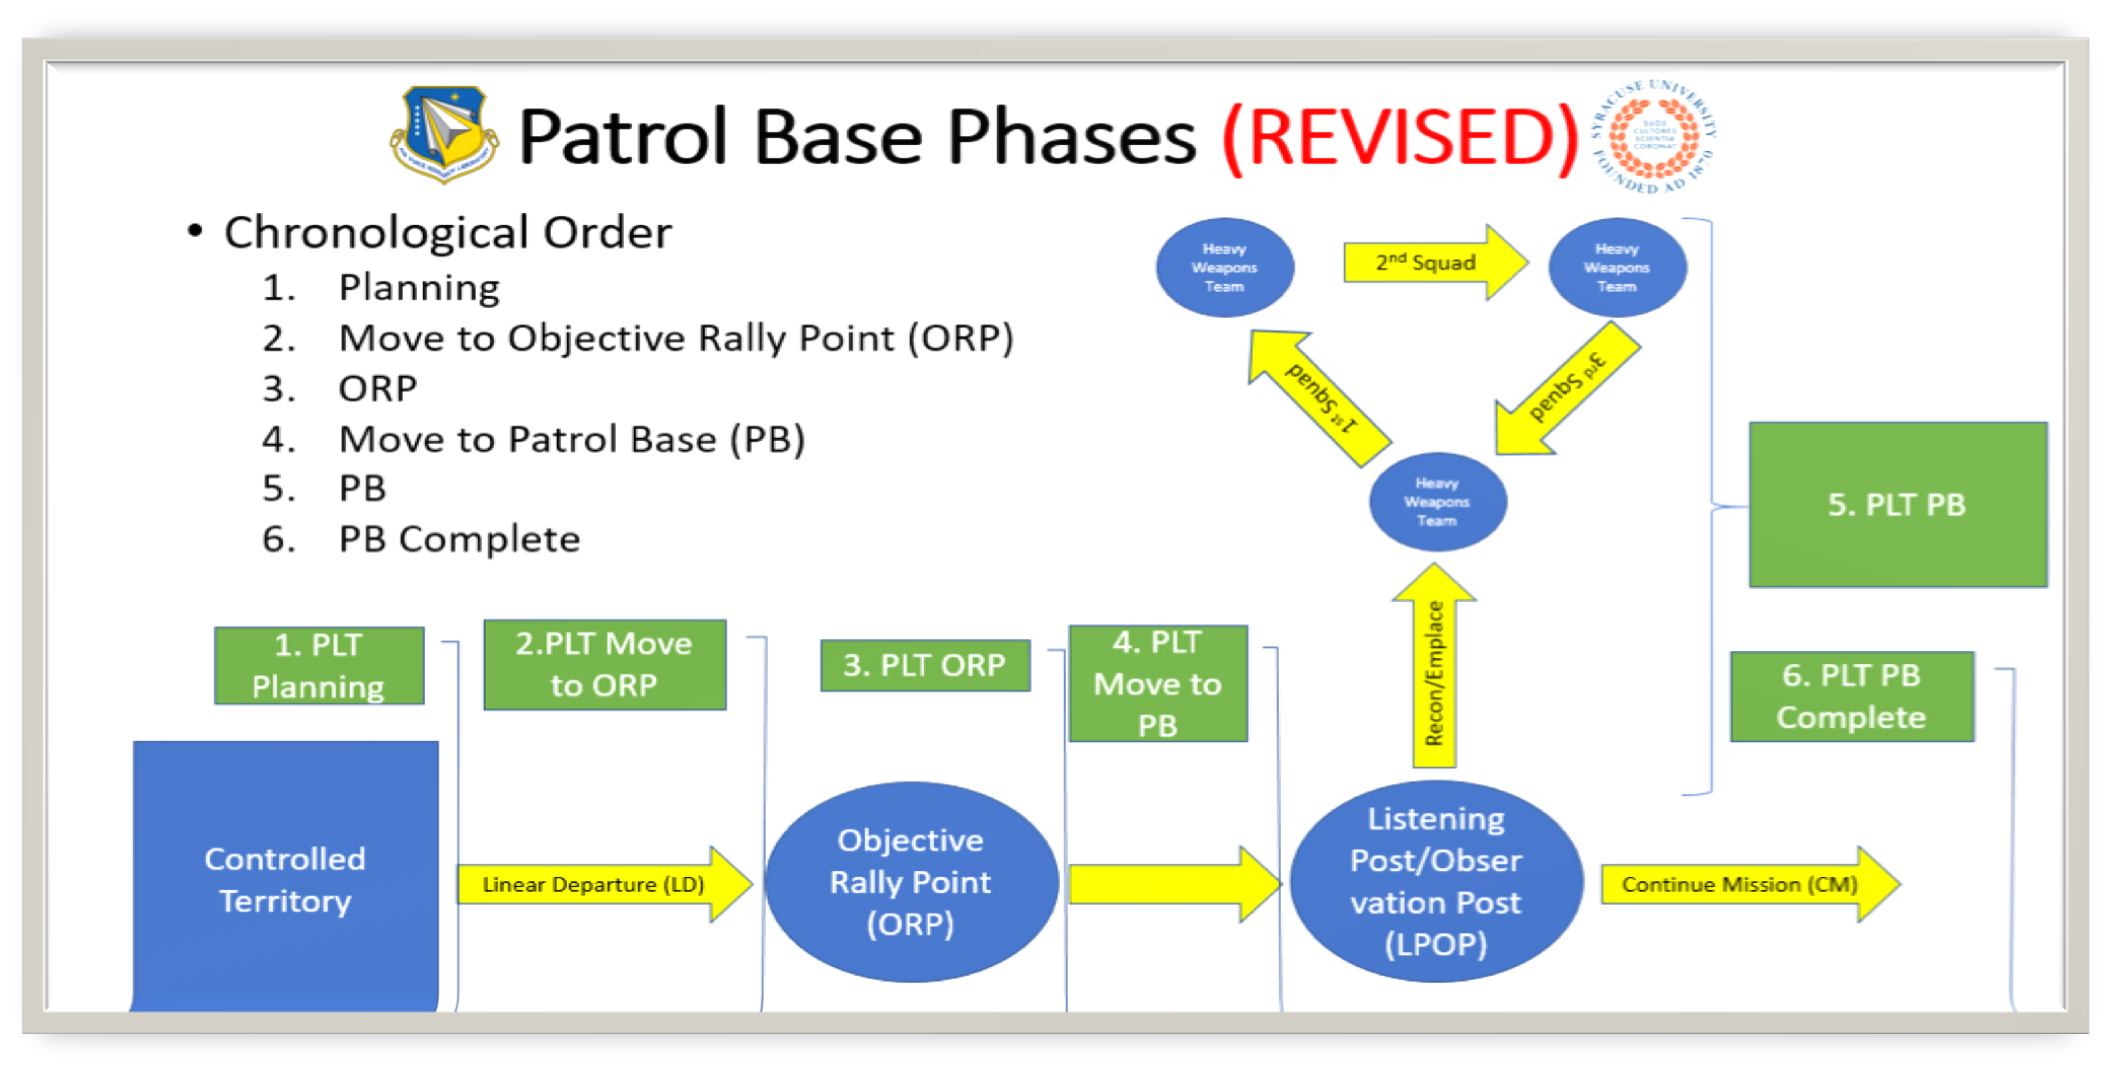
\includegraphics[width=\textwidth]{../figures/pbtoplevel}
\caption{\label{pbtoplevel}A diagram of the most abstract level in the hierarchy of secure state machines.  Image generated by Jesse Nathaniel as part of the research involved in this master thesis.  Shall I get his permission?}
\end{figure}

The diagram describes a chronological order of abstract phases (modeled as states) of the patrol base operations.  The operations begin with the planning phase (1).  Next, they move to the objective rally point (\glsentryshort{orp}) (2). At the \glsentryshort{orp}, operations commence (3).  When these are complete, the patrol base operations move to the actual patrol base (4).  At the patrol base, operations proceed (5).  Finally, the patrol base operations are complete (6).  These are the six states in the top level \glsentryshort{ssm}.


The next level of abstraction in the hierarchy of \glsentryshortpl{ssm} represents a horizontal slice through the patrol base operations.  This is the second level of the hierarchical description of the patrol base operations. It is referred to as the sub level.  In this documentation, \glsentryshortpl{ssm} at this level are referred to as the sub-level, sublevel, or subLevel \glsentryshortpl{ssm}. This slice describes the patrol base operations at a lower level of abstraction.  It expands each of the states in the top level (except for the last state PB Complete).  For example, the planning phase (1) in figure \ref{pbtoplevel} is expanded into an \glsentryshort{ssm} of its own.  This is called ssmPlanPB.  It consists of several states (see section \ref{sssec:ssmPlanPB}) which detail activities conducted during the planning phase of the patrol base operations.  Each state in the top level (except for PB Complete) has it's own \glsentryshort{ssm} (see the next section).

At yet another lower level of abstraction is the sub-sub (3rd) level.  In this documentation, \glsentryshortpl{ssm} at this level are referred to as the sub-sub-level, subsublevel, or subsubLevel \glsentryshortpl{ssm}.  This level expands upon the states in the sub level (one level above) in the same manner that the sub level expands upon the states in the top level \glsentryshort{ssm}.  In this manner, each level is a lower level of abstraction than the level above it. 

A vertical slice through the diagram is also modeled.  This slice models the patrol base operations from the top level down to the most detailed level (level 8).  This vertical slice consists of a series of \glsentryshortpl{ssm}.  Each \glsentryshort{ssm} expands upon only one state in the level above it.  This differs from the horizontal slice which expands upon all states in the level above it.  Expanding upon only one state focuses on a vertical slice through all 8 states of the hierarchy of \glsentryshortpl{ssm}.

The vertical slice begins at the top level \glsentryshort{ssm}.  Next, it expands upon one state at this level, the \textit{move to ORP} state (2).  This results in a sub level \glsentryshort{ssm} named ssmMoveToORP.  The vertical slice progresses in this manner, by expanding one state at each level into a new \glsentryshort{ssm}.  From ssmMoveToORP, the state \textit{secure halt} is expanded to ssmSecureHalt.  From within this \glsentryshort{ssm}, the state \textit{ORP Recon} is expanded into ssmORPRecon.  From within this \glsentryshort{ssm}, the state \textit{Move to ORP 4L} (fourth level move to ORP state) is expanded into ssmMoveToORP4L.  Finally, from within this \glsentryshort{ssm}, the state \textit{Form RT} is expanded into ssmFormRT.

The vertical slice spans the all eight levels.  However, not all levels are represented with an \glsentryshort{ssm}.  The last \glsentryshort{ssm} in the vertical slice, ssmFormRT, is actually at the 5th level of the hierarchy.  This \glsentryshort{ssm}, consists of three states.  These three states reside at the 7th level because ssmFormRT does not have states at the 6th level (it skips the 6th level).  Furthermore, the 7th level states are not expanded into an \glsentryshort{ssm} because each of these 7th level states expand into only one state at the 8th level.  

In addition to the horizontal and vertical slices, an escape level is also modeled.  Actions in the escape level are reachable from any phase of the patrol base operations.  These actions are the unacceptable circumstances that require the patrol base operations to abort.  For example, if the patrol base contacts the enemy in any phase of the operations, then the command \textit{react to combat} is issued.  The patrol base operations are subsequently aborted.  

Excluding the escape level, there are eight levels of the hierarchy of \glsentryshortpl{ssm}.

Note that, the purpose of this master thesis is to demonstrate that the properties of complete mediation could be applied and verified on a non-automated, human-centered systems. Thus, it is sufficient to demonstrate this on a horizontal and vertical slice of the patrol base operations.  

   %%%%%%%%%%%%%%%%%%% Section Hierarchy of Secure State Machines %%%%%%%%%%
\section{Hierarchy of Secure State Machines}
\begin{figure}[h]
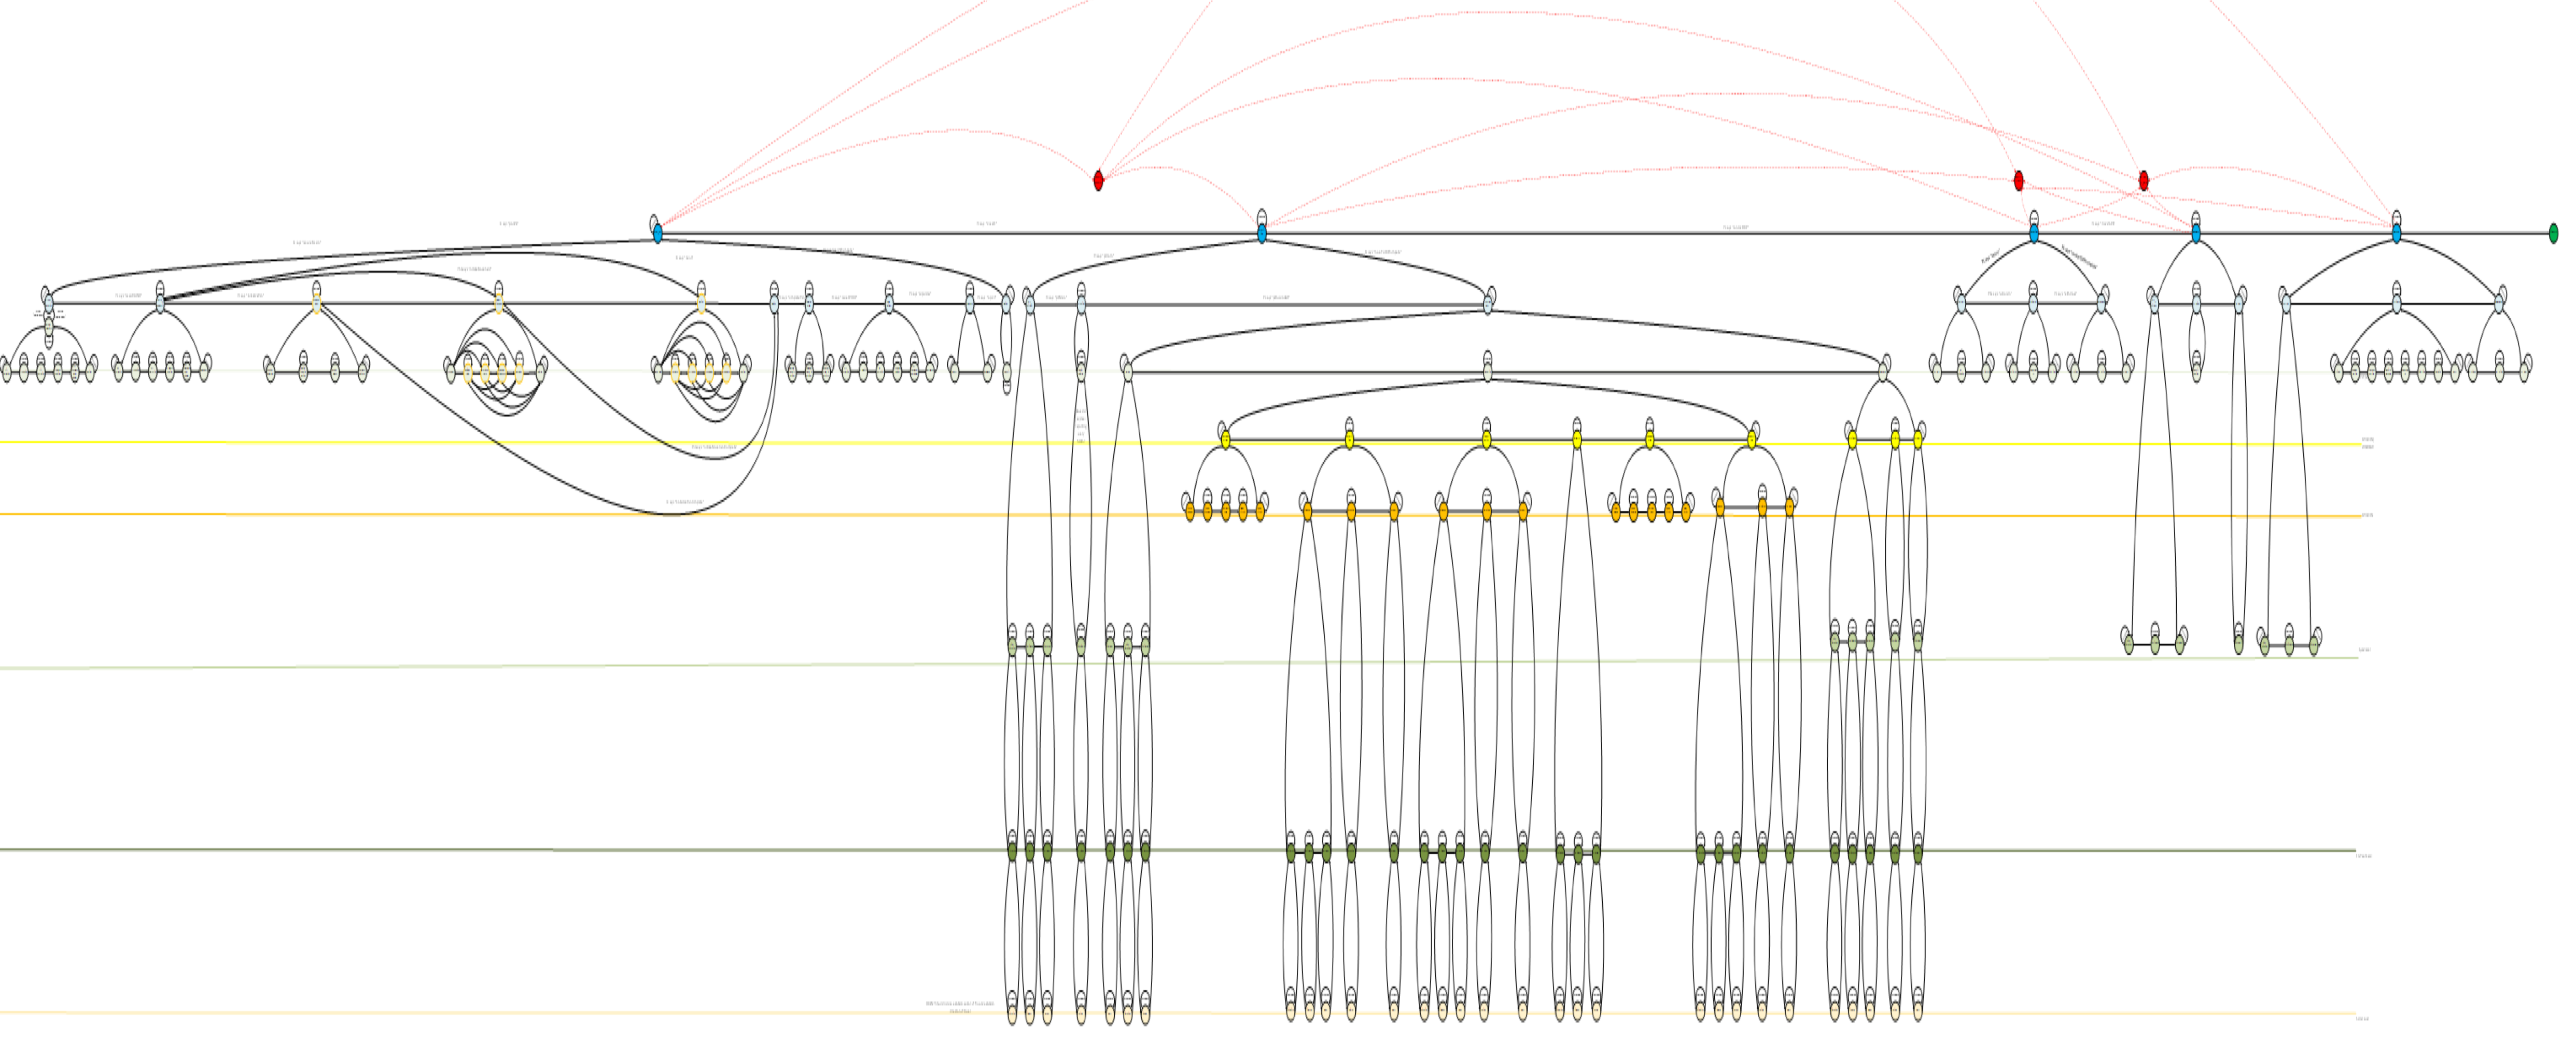
\includegraphics[width=\textwidth]{../figures/overalldiagramsquashed.png}
\caption{\label{overalldiagramsquashed}Diagrammatic description of patrol base operations as a hierarchy of secure state machines.  (Generated by Jesse Nathaniel Hall.)}
\end{figure}

          %%%%%%%%%%%%%%%% Subsection Diagrammatic Description %%%%%%%%%%%%%%
\subsection{Diagrammatic Description in Visio}\label{ssec:overalldiagram}
The enormity of the hierarchy of \glsentryshortpl{ssm} is evident in figure \ref{overalldiagramsquashed}.  This is a squashed version of the Visio diagram for the hierarchy of \glsentryshortpl{ssm}. The diagram is included as a Visio file with the files for this project (LaTeX/figures/diagram.vis).  

The straight, colored lines that span the diagram in figure \ref{overalldiagramsquashed} delineate levels of the hierarchy of \glsentryshortpl{ssm}.  The top lines are obscured by the size of this squashed version of the diagram.  The most visible bright yellow line delineates the sub-sub-sub (4th) level of the hierarchy, for example.


The small, colored dots in figure \ref{overalldiagramsquashed} represent states (phases) of the patrol base operations.  The red dots are an exception.  The labels for these states are not readable in this diagram.  The dots are color coded.  The colors correspond to the level of those states.  For example, the dots at the top level (level below the red dots) are all dark blue.  

In figure \ref{overalldiagramsquashed}, the red dots at the top of the diagram represent the escape level \glsentryshort{ssm}.  But, they do not represent states in the \glsentryshort{ssm}.  This is because the escape level  \glsentryshort{ssm} is accessible by all phases of the patrol base operations.  This means that if can not be ascribed to any one level of the hierarchy. 


The dots representing states are connected to each other by lines.  These lines represent allowable transitions from one state to another.  The escape level is again an exception.  If no line connects one state to another then no transition is allowed.  

The red dots representing the escape level \glsentryshort{ssm} are best thought of as multiple copies of a floating \glsentryshort{ssm}.  The escape level \glsentryshort{ssm} acts as a sub-\glsentryshort{ssm} for all \glsentryshortpl{ssm} in the hierarchy.  During patrol base operations, abortion of the patrol base operations can occur at any action from any state at any level.  This means that any state at any level can be terminated by the escape level \glsentryshort{ssm}.  Drawing lines from all states to the escape level \glsentryshort{ssm} and drawing really long lines clutters the diagram.  Therefore, only lines at the top level are drawn and the red dots are duplicated.

 The lines in the diagram are annotated by \glsentryshort{ssm} requests.  (Annotations are visible in the original Visio diagram, but not in this squashed version.)  For example, a line connecting the top level state PLAN_PB is annotated with the request \textit{PlatoonLeader says crossLD}.  crossLD is an abbreviation for "cross the line of discrimination" and it is the command to transition to the MOVE_TO_ORP state.    Lines are not annotated beyond the sub level.

Details of each level follow in the next section.  
 

          %%%%%%%%%%%%%%%% Subsection OMNI-Level %%%%%%%%%%%%%%%%%%%%%
\subsection{OMNI-Level}\label{ssec:omnilevel}

          %%%%%%%%%%%%%%%% Subsection Escape %%%%%%%%%%%%%%%%%%%%%%%
\subsection{Escape}\label{ssec:escape}

          %%%%%%%%%%%%%%%% Subsection Top Level %%%%%%%%%%%%%%%%%%%%%%
\subsection{Top Level}\label{ssec:toplevel}

          %%%%%%%%%%%%%%%% Subsection Horizontal Slice %%%%%%%%%%%%%%%%%%%
\subsection{Horizontal Slice}\label{ssec:horizontalslice}

                  %%%%%%%%%%%%% Subsection ssmPlanPB %%%%%%%%%%%%%%%%%%%%%
\subsubsection{ssmPlanPB}\label{sssec:ssmPlanPB}

                  %%%%%%%%%%%%% Subsection ssmMoveToORP %%%%%%%%%%%%%%%%%%%
\subsubsection{ssmMoveToORP}\label{sssec:ssmMoveToORP}

                  %%%%%%%%%%%%% Subsection ssmConductORP %%%%%%%%%%%%%%%%%%
\subsubsection{ssmConductORP}\label{sssec:ssmConductORP}

                  %%%%%%%%%%%%% Subsection ssmMoveToPB %%%%%%%%%%%%%%%%%%%
\subsubsection{ssmMoveToPB}\label{sssec:ssmMoveToPB}

                  %%%%%%%%%%%%% Subsection ssmConductPB %%%%%%%%%%%%%%%%%%%
\subsubsection{ssmConductPB}\label{sssec:ssmConductPB}

          %%%%%%%%%%%%%%%% Subsection Vertical Slice %%%%%%%%%%%%%%%%%%%%
\subsection{Vertical Slice}\label{ssec:verticalslice}

                  %%%%%%%%%%%%% Subsection ssmSecureHalt %%%%%%%%%%%%%%%%%%%
\subsubsection{ssmSecureHalt}\label{sssec:ssmSecureHalt}

                  %%%%%%%%%%%%% Subsection ssmORPRecon %%%%%%%%%%%%%%%%%%%
\subsubsection{ssmORPRecon}\label{sssec:ssmORPRecon}

                  %%%%%%%%%%%%% Subsection ssmMoveToORP4L %%%%%%%%%%%%%%%%%
\subsubsection{ssmMoveToORP4L}\label{sssec:ssmMoveToORP4L}

                  %%%%%%%%%%%%% Subsection ssmFormRT %%%%%%%%%%%%%%%%%%%%
\subsubsection{ssmFormRT}\label{sssec:ssmFormRT}


\end{document}